\documentclass[10pt,a4paper]{report}
\usepackage[utf8]{inputenc}
\usepackage[czech]{babel}
\usepackage[T1]{fontenc}
\usepackage{amsmath}
\usepackage{amsfonts}
\usepackage{mwe}
\usepackage{amssymb}
\usepackage{graphicx}
\usepackage{subcaption}
\author{Pavla Kratochvílová, Adriana Šmijáková}
\title{IV109 - Formace názorů}

\begin{document}
\maketitle
% stručné uvedení do tématu, objasnění základních pojmů
\chapter{Úvod}

\chapter{Návrh modelu}
% přesná formulace modelovaného problému, případná relevantní data
\section{Formulace problému}
Naším cílem je zachytit proces formování názorů, který probíhá při interakcích lidí v sociální síti. Vycházíme z myšlenky, že názory člověka jsou do značné míry ovlivněny názory v jeho okolí. Uvažujeme přitom spojitý názor -- člověk nemusí pouze zcela přijmout nebo zamítnout názor svého okolí, ale může jen lehce poupravit svůj vlastní názor tak, aby se více přiblížil názoru okolí. 

Formování názorů zkoumáme na několika různých typech sítí a s různým počátečním rozložením názorů. 

% popis zvoleného přístupu k modelování a základních prvků modelu, vztahů a zpětných vazeb, vysvětlení základních rovnic/pravidel
\section{Model}
Formování názorů modelujeme pomocí agentů, kdy každý agent má přidělen názor vyjádřený reálným číslem z intervalu $\langle 0, 1 \rangle$. Agenti jsou vzájemně propojeni v rámci určitého grafu a interagují spolu pouze agenti spojení vazbou.

Model se skládá ze dvou částí: nejprve se vytvoří síť agentů a každému se nastaví názor, a poté probíhá samotný proces formování názorů.

\subsection{Tvorba grafu}
Všechny grafy jsou parametrizovány počtem vrcholů (parametr \texttt{people}) a průměrným stupněm vrcholů (parametr \texttt{average-node-degree}). Uvažovali jsme čtyři různé typy grafů:

\begin{itemize}
	\item Náhodný graf vzniká náhodným přidáváním hran, dokud neodpovídá průměrný stupeň vrcholů.
	\item Prostorový graf (spatial graph) je převzatý z již existujícího modelu \textit{Virus on a Network}. Je vytvořen náhodným rozmístěním agentů do prostoru a následným přidáváním hran, dokud neodpovídá průměrný stupeň vrcholů. Hrany jsou přidávány mezi náhodným agentem a jemu nejbližším agentem, se kterým ještě není spojen.
	\item Malý svět je založený na existujícím modelu \textit{Small World}. Nejprve je vytvořen cyklus všech agentů, a poté jsou přidány hrany mezi agenty vzájemně vzdálenými méně než nějaké n tak, aby se stupeň vrcholu co nejvíce přiblížil zvolenému průměrnému stupni. Následně některé hrany zamění jeden svůj konec za náhodný jiný. Počet takových hran je dán nepřímo parametrem \texttt{rewiring-prob}.
	\item Preferenční graf je založený na existujícím modelu \textit{Prefferential Attachment}. Vzniká postupným přidáváním vrcholů, přičemž nový vrchol se spojí s nějakým již existujícím. Upřednostňovány jsou vrcholy, které mají více hran -- toho je dosaženo náhodným výběrem z konců hran raději než výběrem z vrcholů. V preferenčním grafu se parametr \texttt{average-node-degree} nebere v úvahu.
\end{itemize}

Výběr typu grafu lze provést pomocí parametru \texttt{network-type}.

\subsection{Počáteční rozložení názorů}
Agentům jsou přiřazeny názory v intervalu $\langle 0, 1 \rangle$. Uvažovali jsme tři možná počáteční rozložení názorů:

\begin{itemize}
	\item Uniformní rozložení.
	\item Normální rozložení -- s průměrem $0.5$ a standardní odchylkou $0.2$.
	\item Normální rozložení se středem v extrémech -- stejné jako normální rozložení v předchozím bodě, ale posunuté tak, aby nejvíce názorů bylo extrémních (tj. těsně nad $0$ a těsně pod $1$) a nejméně středových (tj. okolo $0.5$).
\end{itemize}

Počáteční rozložení názorů lze změnit pomocí parametru \texttt{opinion-distribution}. 

\subsection{Změny názorů}
Uvažujeme dvě strategie pro změnu názorů:

\begin{itemize}
	\item Jeden soused -- agent se podívá na jednoho náhodného agenta ze svého okolí a podle jeho názoru změní svůj vlastní názor.
	\item Všichni sousedé -- agent se podívá na všechny agenty ve svém okolí a podle jejich průměrného názoru změní svůj vlastní názor.
\end{itemize}

V obou případech proběhne změna názoru stejným způsobem. Agent nejprve vypočte rozdíl mezi svým názorem a názorem okolí (tj. buď názor vybraného souseda, nebo průměrný názor všech sousedů), a následně posune svůj názor o zlomek tohoto rozdílu směrem k názoru okolí. Velikost zlomku je daná parametrem \texttt{changing-opinion-strength} (sila změny názoru).

\chapter{Simulace a analýza}
Model preberania názorov sme navrhli tak, že agenti sa snažia prispôsobiť okoliu, preto výsledok dlhodobého behu simulácie nie je zaujímavý. Pokiaľ je graf spojitý, agenti zo začiatku rýchlo konvergujú k nejakému spoločnému názoru, zhode a tým je zvyčajne hodnota pohybujúca sa v okolí $0.5$. Z toho dôvodu v analýze skúmame skôr priebeh formovania názorov namiesto pozorovnania konečného stavu. V tejto kapitole si rozoberieme vplyv parametrov na priebeh správania modelu.

\section{Sila zmeny názoru}

Silu zmeny názoru sme simuláciou skúmali pomocou premennej \i{zmena}(changes v obrázkoch), ktorá určuje súčet všetkých zmien medzi súčasným a predchádzajúcim časovým okamihom naprieč všetkými osobami. Keďže je tento súčet ovplyvnený samotnou hodnotou parametru \texttt{changing-opinion-strength}, na obrázku 3.1(b) je hodnota normovaná. Na obrázku 3.2 vidíme porovnanie zmeny \texttt{changing-opinion-strength} pre rôzne grafy. Obrázky 3.1 aj 3.2 vznikli spriemerovaním $10$ behov s rovnako nastavenými parametrami. Grafy obsahujú zakaždým $100$ ľudí s priemerným stupňom vrcholu $7$ (okrem preferenčného grafu), stratégiou rozhodovanie \texttt{one neighbor} a uniformným počiatočným rozdelením. Graf typu Malý svet má ktomu nastavenú pravdepodobnosť predrátovania na 30\%, pri ktorej je priemerná najkratšia cesta medzi vrcholmi približne rovnaká ako pre preferenčný graf. Skúmané vlastnosti v tejto časti môžme pozorovať na popísaných obrázkoch.  

Pokiaľ je nastavená sila zmeny názoru na hodnotu $0.5$, model sa najrýchlejšie ustáli na jednotmon názore. Ako sa však posúva ku $0$ alebo $1$, zmeny v názoroch trvajú dlhšie a sú výraznejšie. Najdlhšie trvá ustálenie názoru pre hodnotu $1$ ale tento prípad je odlišný od zvyšku hodnôt a to tým, že počas simulácie prestávajú ľudia upravovať len čiastočne ale preberú výsledný názor, ktorý im vznikne podľa vybranej stratégie (pre \texttt{one neighbor} preberú úplne názor nejakého zo susedov, pre \texttt{all neighbors} majú presnú hodnotu priemeru všetkých susedov). Hodnota $1$ je zároveň jediná kde je možné sledovať za nastavenia stratégie jedného suseda sledovať inú výslednú hodnotu ako blízku hodnote $0.5$.

\begin{figure}
\begin{subfigure}{.5\textwidth}
  \centering
  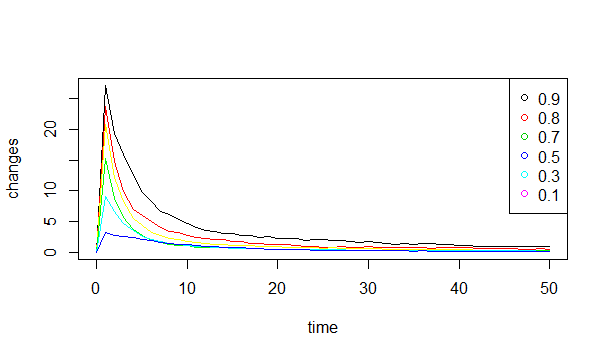
\includegraphics[width=1\linewidth]{plots/spatial-g/spatialChanges1-9.png}
  \caption{Nenormovaný graf}
  \label{fig:sfig1}
\end{subfigure}%
\begin{subfigure}{.5\textwidth}
  \centering
  
  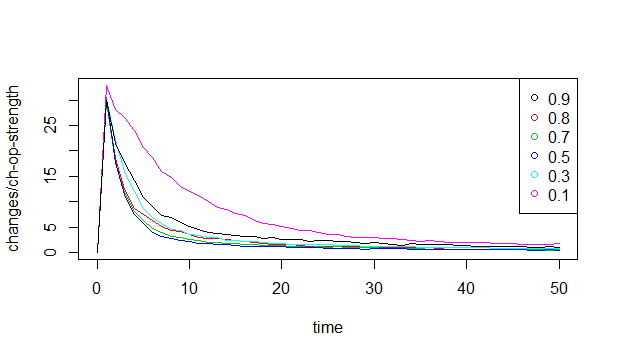
\includegraphics[width=1\linewidth]{plots/spatial-g/spatialChanges1-9norm.png}
  \caption{Normovaný graf}
  \label{fig:sfig2}
\end{subfigure}
\caption{Priestorový graf - vývin zmien s parametrom \texttt{changing-opinion-strength} v rozpätí $0.1$ - $0.9$}
\label{fig:fig}
\end{figure}


Ďalším pozorovaním vyplynulo, že pri hodnotách menších ako 0.5 sú zmeny výraznejšie a dlhotrvajúcejšie ako pri hodnotách rovnako vzdialených od $0.5$ ale smerom k jednotke. Pokiaľ opomenieme hraničné hodnoty $0$ a $1$, sila zmeny názoru $0.1$ je najviac výrazná. Na obrázku 3.1(b) vidno, že pod touto hodnotou trvá zhoda najdlhšie a zároveň najväčší počet ľudí mení názor.


\begin{figure*}
  \centering
  \begin{subfigure}[b]{0.475\textwidth}
      \centering
      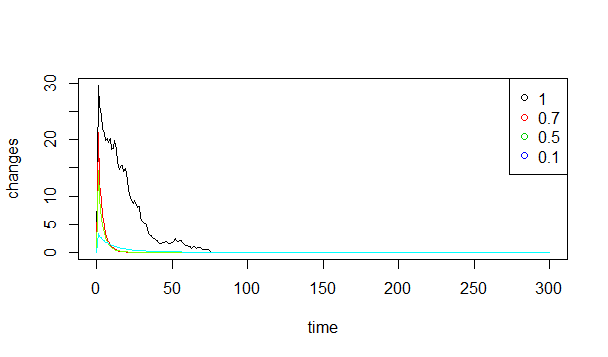
\includegraphics[width=\textwidth]{plots/random-g/changesRandom.png}
      \caption[Network2]%
      {{\small Náhodný graf}}    
      \label{fig:mean and std of net14}
  \end{subfigure}
  \hfill
 \begin{subfigure}[b]{0.475\textwidth}   
      \centering 
      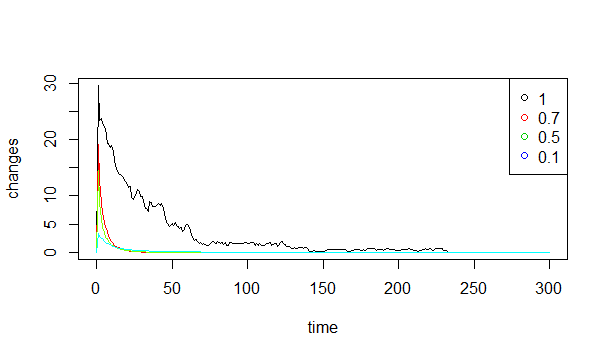
\includegraphics[width=\textwidth]{plots/small-world-g/changesSmallWorld.png}
      \caption[]%
      {{\small Priestorový graf}}    
      \label{fig:mean and std of net34}
  \end{subfigure}
  \vskip\baselineskip
  
    \begin{subfigure}[b]{0.475\textwidth}  
      \centering 
      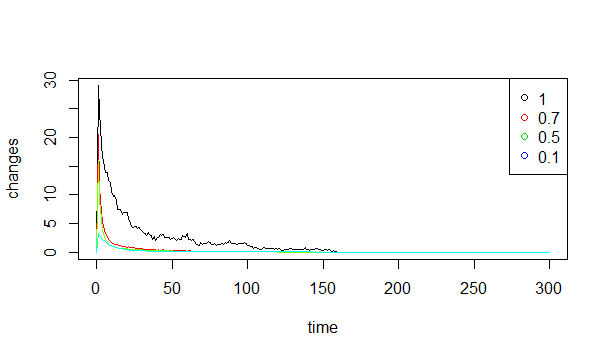
\includegraphics[width=\textwidth]{plots/spatial-g/ChangesOneSpatial.png}
      \caption[]%
      {{\small Malý svet}}    
      \label{fig:mean and std of net24}
  \end{subfigure}
  \quad
  \begin{subfigure}[b]{0.475\textwidth}   
      \centering 
      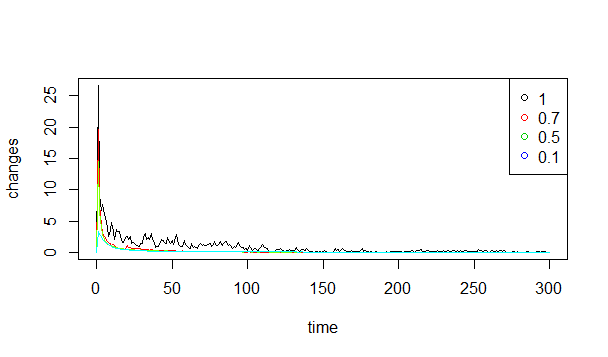
\includegraphics[width=\textwidth]{plots/prefferential-g/changesPrefferential.png}
      \caption[]%
      {{\small Preferenčný graf}}    
      \label{fig:mean and std of net44}
  \end{subfigure}
  \caption[ Vývin zmien pre jednotlivé grafy so zmenou parametru ]
  {\small Vývin veľkosti zmien názorov pre jednotlivé grafy s parametrom \texttt{changing-opinion-strength}}
  \label{fig:mean and std of nets}
\end{figure*}
Keď porovnáme rôzne grafy, pozorujeme len malé zmeny pre $\texttt{changing-opinion-strength} < 1$. Rozdiel vidíme najviac pri spomenutej hodnote 1, vynikajú najmä preferenčný a náhodný graf. V preferenčnom grafe sa veľmi rýchlo názory rozšíria a následne už len malý počet ľudí mení názory v omnoho dlhšom časovom horizonte v porovnaní s inou topológiou, priestorový graf je týmito vlastnosťami podobný ale nie až tak výrazný. V náhodnom grafe sa ľudia zase najrýchlejšie zhodnú a ďalej sa stav nemení.

Pri popise ďalších parametrov sme už nepoužívali nastavenie $\texttt{changing-opinion-strength} = 1$ práve kvôli tomu, že zmení charakter modelu (rozdelenie na spojitý názor prestáva mať zmysel zároveň so stratégiou jedného suseda a problém sa dá pozorovať ako n diskrétnych názorov).

\section{Počáteční rozložení názorů}
Normálne rozdelenie s průměrem $0.5$ a standardní odchylkou $0.2$ má oproti zvyšným dvom podstatne väčší dopad na vývin zmien názorov. Na obrázku 3.3 vidíme vplyv rôzneho nastavenia počiatočného rozloženia názorov, konkrétne pre náhodní graf so silou zmeny názoru $0.1$. Keďže z povahy modelu sa blížia názory ľudí k okoliu hodnoty $0.5$, toto rozdelenie urýchli konvergenciu k tejto hodnote.
\begin{figure}
  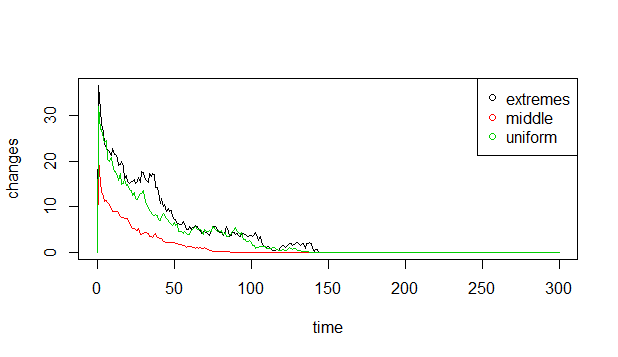
\includegraphics[width=\textwidth]{plots/small-world-g/smallWorldDistribution.png}
  \caption{Vývin veľkosti zmien s parametrom \texttt{opinion-distribution} }
\end{figure}


\section{Stratégia zmeny názoru}
Podobne ako počiatočné normálne rozdelenie názorov, stratégia zmeny názoru zohľadnenia názoru všetkých susedov urýchľuje ustálenie jednotného názoru. Tento trend ukazuje obrázok 3.4, ktorý je vytvorený nad priestorovým grafom so silou zmeny názoru $0.1$.  
\begin{figure}
  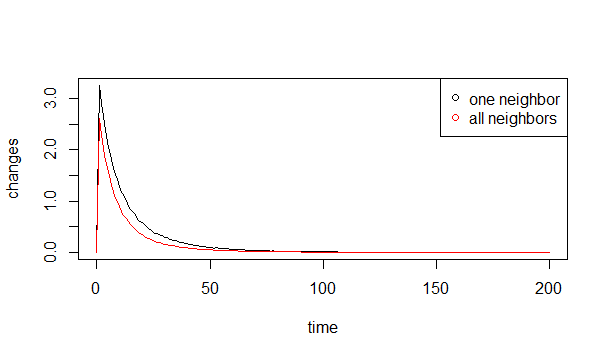
\includegraphics[width=\textwidth]{plots/random-g/randomAllVsOne.png}
  \caption{Vývin veľkosti zmien s parametrom \texttt{opinion-distribution} }
\end{figure}

\section{Typ grafu}
Zmeny v chovaní modelu pri rôznej topológii sme mohli vidieť už na obrázku 3.1, ktorý bol rozobratý v kapitole 3.1, avšak nevypovedal o konkrétnych hodnotách názorov. Priebeh zmien hodnôt môžme vidieť na obrázku 3.5. Znázorňuje názory nachádzajúce sa v určitom percentuálnom umiestnení v spektre hodnôt od najnižšej (0\%) po najvyššiu (100\%). Stredná hodnotá má na obrázku hodnotu 50\%. Oproti ostatným, tento obrázok nevznikol spriemerovaním hodnôt z viacerých behov ale znázorňuje len priebeh v jednom behu pre každý typ grafu. Napriek tomu pozoruje podobné vlastnosti medzi priestorovým a preferenčným grafom podobne ako v prípade obrázku 3.1. V náhodnom grafe a malom svete zase názory veľmi rýchlo splinú do jedného s hodnotou v okoli $0.5$.

\begin{figure*}
  \centering
  \begin{subfigure}[b]{0.475\textwidth}
      \centering
      \includegraphics[width=\textwidth]{plots/max-values/random-MaxV.png}
      \caption[Network2]%
      {{\small Náhodný graf}}    
      \label{fig:mean and std of net14}
  \end{subfigure}
  \hfill
  \begin{subfigure}[b]{0.475\textwidth}  
      \centering 
      \includegraphics[width=\textwidth]{plots/max-values/spatial-MaxV.png}
      \caption[]%
      {{\small Priestorový graf}}    
      \label{fig:mean and std of net24}
  \end{subfigure}
  \vskip\baselineskip
  \begin{subfigure}[b]{0.475\textwidth}   
      \centering 
      \includegraphics[width=\textwidth]{plots/max-values/small-world-MaxV.png}
      \caption[]%
      {{\small Malý svet}}    
      \label{fig:mean and std of net34}
  \end{subfigure}
  \quad
  \begin{subfigure}[b]{0.475\textwidth}   
      \centering 
      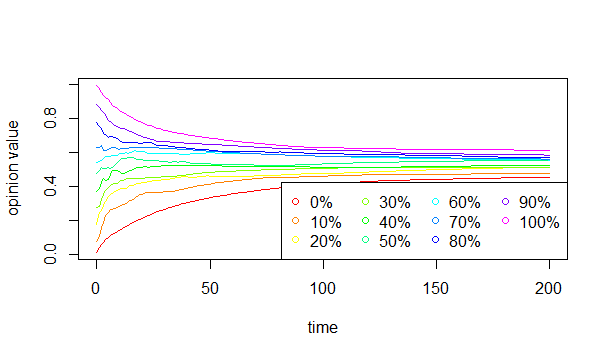
\includegraphics[width=\textwidth]{plots/max-values/prefferentialMaxV.png}
      \caption[]%
      {{\small Preferenčný graf}}    
      \label{fig:mean and std of net44}
  \end{subfigure}
  \caption[ Vývin zmien pre jednotlivé grafy ]
  {\small Vývin hodnôt názorov pre jednotlivé grafy}
  \label{fig:mean and std of nets}
\end{figure*}
 
\chapter{Závěr}

\end{document}